\section{成本感知的选择性分离规划}
\sectionen{Cost-Aware Planning for Selective Disaggregation}
\label{sec:planning}

\subsection{Motivation}
不同请求从分离执行中得到的收益并不相同。较长的输入可能值得交给专门的 P 池，较短的输入则可能更适合留在 M 池。规划器需要同时选择分流阈值、角色数量和频率：既让适合分离的请求获益，又保留完整部署的能量收益。这里的选择发生在两个层次：周期性比较资源方案，再按选定规则逐请求分流。
\EN{Requests benefit differently from disaggregation. Longer prompts may justify a dedicated P pool, while shorter prompts may be better served by M instances. The planner jointly selects the routing threshold, role counts, and clocks to turn these differences into deployment-level energy savings. It compares resource plans periodically; individual requests then follow the selected routing rule.}

\subsection{Challenge}
阈值改变两条路径的请求比例，资源数量和频率又改变各自的排队与服务能力。功率更低的方案可能缺少解码容量；性能可行的方案也可能无法收回交接和配置切换的开销。因此，比较必须使用相同负载、相同能量窗口和相同 SLO 约束，还要把停驻 GPU 计入，避免只挑出某一阶段的优势。
\EN{The threshold changes the load on each path, while replica counts and clocks change queueing and service capacity. A low-power layout can lack decode capacity, and a feasible layout can still save too little to cover handoff and reconfiguration. Compare candidates under the same workload, energy horizon, and SLO constraints, including the GPUs that remain parked.}

\subsection{Insight}
先检查候选是否有模型支持、是否具备足够容量，再比较完整窗口成本。选择性分离不是固定偏好：收益足够时采用，收益不足时保留当前可行方案。规划器把资源配置与阈值作为同一个 Plan 输出；在线层执行它，并将观测反馈给下一轮规划，而不另行改变已经评估的分流比例。
\EN{First check model coverage and capacity, then compare complete window costs. Selective disaggregation is a conditional choice: use it when it saves enough, and retain a feasible current plan when it does not. Resource allocation and threshold belong to one Plan. The runtime executes that Plan and returns observations for the next decision without independently changing the evaluated traffic split.}

\subsection{Approach}
\paragraph{输入与输出 / Inputs and outputs.}
输入为负载估计 $F$、离线模型、SLO、GPU 预算、当前就绪配置 $c$ 和窗口 $H$。负载估计包含到达率以及输入、输出长度统计。输出 Plan 包含 P/D/M 数量、各池频率、停驻状态与阈值 $\tau$；执行器负责将这些决策落实为可用配置。
\EN{Inputs are demand estimate $F$, offline models, SLOs, the GPU budget, ready configuration $c$, and horizon $H$. Demand includes arrival rate and input/output length statistics. A Plan specifies P/D/M counts, pool clocks, parking states, and threshold $\tau$. The executor turns that Plan into an available configuration.}

\paragraph{比较步骤 / Candidate comparison.}
枚举全 M 与 P/D/M 候选，按 $\tau$ 计算两条路径的负载。没有匹配模型支持的候选先排除，再检查时延、吞吐和 KV 容量。目标模型分别约束用户可见的首 token 延迟与 P--D 续接表现。对可行方案计算：
\begin{equation}
  J(x)=H\,P(x)+E_{\mathrm{extra}}(x,H)+E_{\mathrm{switch}}(c,x).
\end{equation}
$P(x)$ 包含运行与停驻功率；后两项仅计尚未包含的交接增量与本次切换增量，不重复计算基础能量或历史成本。当前方案同样重新评估，且切换到自身的成本为零。
\EN{Enumerate mixed-only and P/D/M candidates, then split demand using $\tau$. Reject unsupported candidates before checking latency, throughput, and KV capacity. The target model distinguishes visible first-token latency from P--D continuation behavior. Score feasible plans using operating and standby power plus incremental handoff and switching energy. Re-evaluate the current plan as well; switching to itself costs zero.}

\begin{figure*}[t]
  \centering
  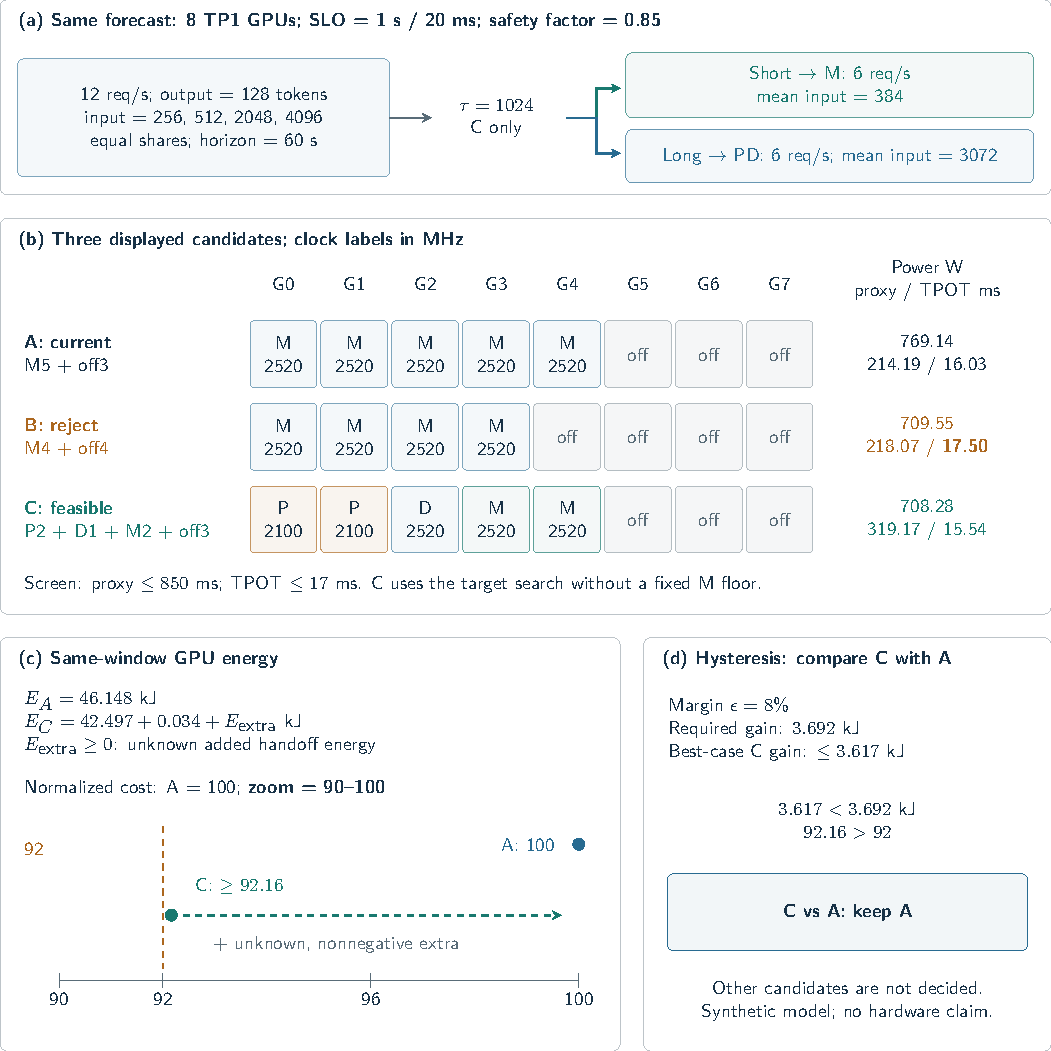
\includegraphics[width=\textwidth]{figures/03-planning.pdf}
  \caption{\textbf{候选筛选与滞回的可复算方法例。}统一使用仓库合成模型，展示三个候选而非完整搜索。B 的预测 TPOT 超过安全筛选线；C 的运行功率较低，但即使额外交接能量为零，替代 A 的收益仍不足 8\%。因此本次 \emph{C 对 A} 的比较保持 A，不对其他未展示候选作出结论。C 的 M2 配置属于取消固定 M 下界后的目标设计。图中时延列为当前规划模型的 \emph{latency proxy}，并非 carry 协议的实测 TTFT。\\
  \textbf{A reproducible example of screening and hysteresis.} Values come from the repository's synthetic model. B fails the guarded TPOT constraint. C uses less operating power, but its best-case saving over A is below 8\%; this pairwise comparison retains A. Other candidates are not decided here. M2 belongs to the target search without a fixed M floor. Latency proxies are model outputs, not measured carry-protocol TTFTs.}
  \label{fig:planning}
\end{figure*}

\paragraph{用一个反例说明切换门槛 / A switching decision.}
图~\ref{fig:planning} 的共同负载含短、长输入各 $6$ req/s；仅候选 C 按阈值分配到两条路径。A 与 C 均通过合成模型的性能检查；60 秒内 A 消耗 $46.148$ kJ，C 的运行及停驻能量为 $42.497$ kJ，另有模型估计的 $34$ J 切换成本。尚未测得的交接增量非负，因此 C 的归一化总成本至少为 $92.16$，而 8\% 滞回要求低于 $92$。这一步判断不需要假造未知交接能量，也不意味着其他负载下应拒绝分离。
\EN{The workload contains $6$ req/s of short prompts and $6$ req/s of long prompts. A and C pass the synthetic performance checks. Over 60 seconds, A uses $46.148$ kJ; C needs $42.497$ kJ for operation and standby plus an estimated $34$ J for switching. Unknown extra handoff energy is nonnegative, so C costs at least $92.16$ when A is normalized to $100$. The 8\% margin requires a cost below $92$. This pairwise rejection neither invents missing measurements nor rules out disaggregation under other conditions.}

\begin{algorithm*}[t]
  \caption{SELECTIVE-PD-PLAN}
  \label{alg:planning}
  \begin{algorithmic}[1]
    \Require Demand $F$, models $M$, constraints $S$, budget $B$, ready plan $c$, horizon $H$, margin $\epsilon$
    \State $A \gets \Call{Candidates}{B} \cup \{c\}$ \Comment{include mixed-only and P/D/M layouts}
    \State $V \gets \varnothing$
    \For{each $x\in A$}
      \State $l \gets \Call{Split}{F,x}$ \Comment{use the candidate's threshold and roles}
      \State \textbf{if} not $\Call{Covered}{M,x,l}$ \textbf{then continue}
      \State $z \gets \Call{Predict}{M,x,l}$
      \State \textbf{if} not $\Call{Feasible}{z,S}$ \textbf{then continue}
      \State $J[x] \gets \Call{Energy}{z,H}+\Call{ExtraKV}{z,H}+\Call{Switch}{c,x}$
      \State $V \gets V\cup\{x\}$
    \EndFor
    \State \textbf{if} $V=\varnothing$ \textbf{then return} $\Call{Safe}{c,M,B}$
    \State $b \gets \arg\min_{x\in V} J[x]$ \Comment{ties prefer mixed-only layouts}
    \State \textbf{if} $c\notin V$ \textbf{then return} $b$
    \If{$J[c]-J[b]\leq\epsilon J[c]$}
      \State \Return $c$
    \EndIf
    \State \Return $b$ \Comment{the executor applies the returned Plan}
  \end{algorithmic}
\end{algorithm*}

算法~\ref{alg:planning} 的前置条件是 $c$ 已由在线层安全启动，不接受空配置。覆盖检查同时约束候选使用的形状、频率与拓扑；缺测不能解释为零成本。保守回退优先恢复可用容量，必要时限制准入，不保证任意过载下仍满足 SLO。图中的局部比较用于解释规则，算法则在完整候选集合中选择。
\EN{The online layer supplies a ready initial or active plan $c$; it cannot be null. Coverage includes shapes, clocks, and topology. Missing measurements do not imply zero cost. Conservative fallback prioritizes available capacity and may limit admission without guaranteeing SLOs under arbitrary overload. The figure illustrates a local comparison; the algorithm operates on the full candidate set.}

\implnote{当前默认候选枚举保留 $M\geq\min(4,\text{slots})$，目标设计取消这一固定下界，由覆盖、容量和 SLO 约束选择配置。现有代码已实现枚举、功率预测、切换滞回及阈值输出；统一验证的增量交接能耗，以及分别预测可见 TTFT 与续接表现，仍是目标改进。图中数值来自合成公式，不构成测量覆盖或硬件性能证据。}{The current default search retains at least $\min(4,\text{slots})$ mixed replicas. The target removes this fixed floor and relies on feasibility constraints. Enumeration, power prediction, hysteresis, and threshold output exist today; uniformly validated extra handoff energy and separate visible-TTFT and continuation predictions remain target improvements. Synthetic calculations are not evidence of hardware performance or measured coverage.}
